\documentclass[10pt]{oblivoir}

% ---------------------------------------------- PACKAGE IMPORTS
\usepackage{kotex}
\usepackage{amsmath}
\usepackage{multicol}
\usepackage{fixltx2e}
\usepackage{float}
\usepackage{graphicx}
\usepackage{fullpage}
\usepackage{siunitx}
\usepackage[ruled,vlined]{algorithm2e}
\usepackage{hyperref}
\usepackage{listings}
\usepackage{color}
\usepackage{caption}
\usepackage{indentfirst}
\usepackage{subcaption}
\usepackage{tikz-cd}
\usepackage{chngcntr}
\usepackage{comment}
\usepackage[nameinlink]{cleveref}

% ---------------------------------------------- FIGURE COUNTER SETTINGS
% \counterwithin{figure}{section}

% ---------------------------------------------- CODE AREA SETTINGS
\definecolor{dkgreen}{rgb}{0,0.6,0}
\definecolor{gray}{rgb}{0.5,0.5,0.5}
\definecolor{mauve}{rgb}{0.58,0,0.82}

\lstset{frame=tb,
  language=C++,
  aboveskip=3mm,
  belowskip=3mm,
  showstringspaces=false,
  columns=flexible,
  basicstyle={\small\ttfamily},
  numbers=none,
  numberstyle=\tiny\color{gray},
  keywordstyle=\color{blue},
  commentstyle=\color{dkgreen},
  stringstyle=\color{mauve},
  breaklines=true,
  breakatwhitespace=true,
  tabsize=3
}

% ---------------------------------------------- CLEVERREF SETTINGS
\crefname{figure}{그림}{그림}
\crefname{equation}{식}{식}
\crefname{table}{표}{표}
\crefname{listing}{목록}{목록}
\crefname{section}{절}{절}
\crefname{algorithm}{알고리즘}{알고리즘}

\captionsetup[subfigure]{subrefformat=simple,labelformat=simple}
    \renewcommand\thesubfigure{ (\alph{subfigure})}

% ---------------------------------------------- GENERAL SETTINGS
\setlength{\parindent}{0.3cm} % The first indent width setup

% ---------------------------------------------- CUSTOM COMMANDS
%       GENERAL
\newcommand{\textss}[1]{\scriptsize#1\normalsize}
%       MATHEMATICAL
\newcommand{\abs}[1]{\left|\,#1\,\right|}

% ---------------------------------------------- HEADER
\title{AR 당구}
\author{강승우 \\ 한국기술교육대학교 전자공학과}
\date{2020.10}

% ---------------------------------------------- CONTENT
\begin{document}
\maketitle

\begin{figure}[ht]
    \centering
    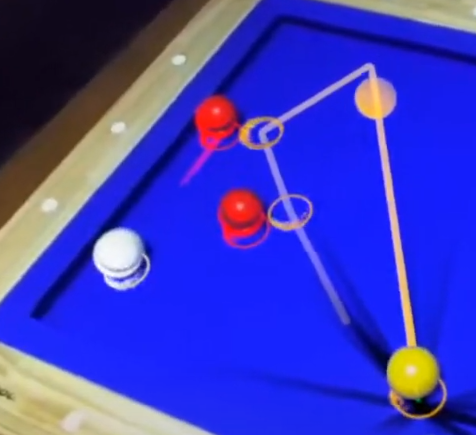
\includegraphics[width=5cm]{img/abstract-final.png}
\end{figure}

\begin{abstract}
    당구는 재미있는 스포츠이지만, 처음 입문한 초심자가 득점 가능한 경로를 계산하고 올바르게 공을 쳐서 보낼 정도로 숙련되기까지의 진입 장벽이 높은 편이다. 당구 초심자가 어느 정도 수준에 도달하기 위해선 지속적인 집중과 훈련을 필요로 하는데, 적절한 동기 부여 요소가 없다면 흥미를 잃어버리기 쉽다. 본 연구는 스테레오 카메라와 VR 카메라를 결합한 몰입도 높은 증강 현실 플랫폼 상에서 당구 경로 안내 및 시각 효과를 통해 초심자의 흥미를 유도하고 당구 학습을 가속하는 것을 목표로 두었다. 이를 위해 OpenCV를 활용하여 당구공 배치를 인식하고 Unity Engine 상에서 물리 시뮬레이션을 통해 경로 탐색과 시각화를 수행하였고, 그 결과 프로그램이 제안한 속도와 방향을 정확히 맞췄을 때 높은 정확도를 보였다. 이는 당구에 처음 입문하는 초심자가 경로 설계에 대한 부담 없이 공을 올바르게 보내는 훈련에만 집중할 수 있게 만들며, 나아가 오랜 시간 알고리즘이 제안하는 경로를 익힘으로써 점진적으로 당구 숙련도를 높일 수 있다는 점에서 AR 당구의 학습 보조 도구로서의 가능성을 확인할 수 있었다.
\end{abstract}

\newpage
\twocolumn[]

\section{서론}

\section{제안 방식}

\section{실험 결과}

\section{결론}

\bibliographystyle{unsrt}
\bibliography{content.bib}

\end{document}
